\documentclass{article}
\usepackage{fancyhdr,booktabs}
\usepackage{amsmath}
\usepackage{float}
\usepackage{graphicx}
\usepackage{indentfirst}
\usepackage{geometry}

\begin{document}

\begin{figure}[!htb]
	\centering
	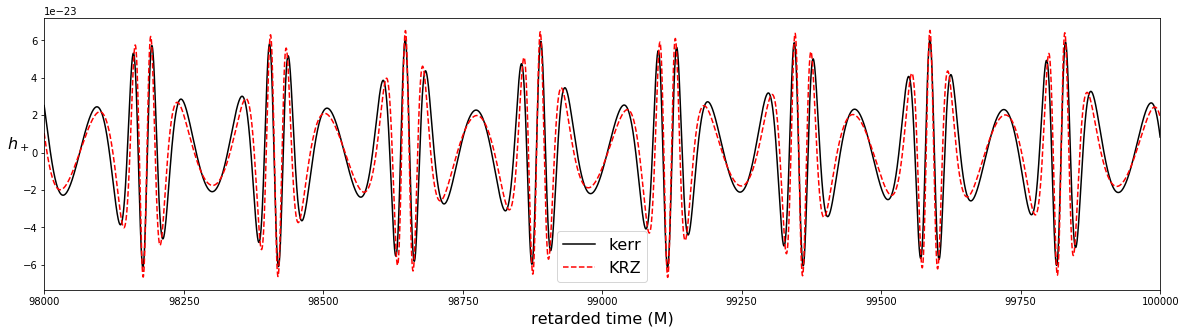
\includegraphics[width=16cm]{krz_kerr_wave.png}
	
	\caption{Comparison between two waveforms of $h_+$ with respect to retarded time in units of central black hole mass $M$. The red dashed line is the waveform under d1=0.2, e=0.5,p=6. The black solid line is the waveform under d1=0 and e, p adapted so that the orbital frequencies $\omega_r$ and $\omega_\phi$ are the same as that of the orbit under d1=0.2, e=0.5, p=6. The spin of the central black hole is 0.5M.}
	\label{range}
\end{figure}	
	
\end{document}